% Korean working manuscript. Layout informed by the supplied LoRA v2 source.
% This file does not claim submission to or acceptance by ICLR.
\documentclass[10pt,letterpaper,twocolumn]{article}
\usepackage[textwidth=7in,textheight=9in,top=1in]{geometry}
\setlength{\columnsep}{0.25in}
\usepackage{fontspec,xeCJK}
\IfFontExistsTF{Times New Roman}{\setmainfont{Times New Roman}}{\setmainfont{TeX Gyre Termes}}
\defaultCJKfontfeatures{Script=Default}
\IfFontExistsTF{AppleMyungjo}{\setCJKmainfont{AppleMyungjo}[AutoFakeBold=2,AutoFakeSlant=.12]}{\IfFontExistsTF{Noto Serif CJK KR}{\setCJKmainfont{Noto Serif CJK KR}}{\setCJKmainfont{NanumMyeongjo}}}
\IfFontExistsTF{AppleGothic}{\setCJKsansfont{AppleGothic}[AutoFakeBold=2]\setCJKmonofont{AppleGothic}}{\setCJKsansfont{Noto Sans CJK KR}\setCJKmonofont{Noto Sans CJK KR}}
\IfFontExistsTF{Menlo}{\setmonofont{Menlo}[Scale=MatchLowercase]}{\setmonofont{Courier New}}
\xeCJKsetup{CJKspace=true}
\XeTeXlinebreaklocale "ko"
\XeTeXlinebreakskip=0pt plus .2pt
\usepackage{amsmath,amssymb,graphicx,booktabs,array}
\usepackage{dblfloatfix}
\usepackage[authoryear,round]{natbib}
\usepackage[font=small,labelfont=bf]{caption}
\usepackage[unicode,hidelinks]{hyperref}
\hypersetup{pdftitle={안전한 모델 위임: 수신 대상별 경로 판단과 전송 본문의 분리 평가},pdfauthor={Junkuk Kim and Jinyoung Choi}}
\renewcommand{\figurename}{그림}
\renewcommand{\tablename}{표}
\renewcommand{\refname}{참고문헌}
\setlength{\parindent}{0pt}
\setlength{\parskip}{5pt plus 1pt minus 1pt}
\setlength{\emergencystretch}{1em}
\setlength{\textfloatsep}{13pt plus 2pt minus 2pt}
\renewcommand{\topfraction}{.92}
\renewcommand{\textfraction}{.08}
\setcounter{topnumber}{2}
\setcounter{dbltopnumber}{2}
\renewcommand{\dbltopfraction}{.92}
\renewcommand{\dblfloatpagefraction}{.7}
\makeatletter
\renewcommand{\section}{\@startsection{section}{1}{\z@}{-2ex plus -.5ex minus -.2ex}{1ex plus .2ex}{\large\bfseries\raggedright}}
\renewcommand{\subsection}{\@startsection{subsection}{2}{\z@}{-1.7ex plus -.4ex minus -.2ex}{.6ex plus .2ex}{\normalsize\bfseries\raggedright}}
\renewenvironment{abstract}{\vspace{3pt}\begin{center}\normalsize\bfseries 요약\end{center}\vspace{-5pt}\begin{quote}\small}{\end{quote}\vspace{3pt}}
\makeatother
\newcommand{\A}{\mathcal{A}}
\newcommand{\R}{\mathcal{R}}
\newcommand{\smalltable}{\small\setlength{\tabcolsep}{3pt}\renewcommand{\arraystretch}{1.13}}
\pagestyle{plain}
\raggedbottom
\clubpenalty=10000
\widowpenalty=10000
\displaywidowpenalty=10000

\begin{document}
\twocolumn[{
\begin{flushleft}
{\fontsize{17}{21}\selectfont\bfseries 안전한 모델 위임: 수신 대상별 경로 판단과\\전송 본문의 분리 평가\par}
\vspace{10pt}
{\large\bfseries Junkuk Kim\textsuperscript{1} \qquad Jinyoung Choi\par}
\vspace{3pt}
{\normalsize\textsuperscript{1}Georgia Institute of Technology\par}
\end{flushleft}
\vspace{3pt}

\begin{abstract}
기업 내부의 로컬 대형 언어 모델(LLM)이 일차 업무를 수행하고 정책이 허용하는 대상과 표현으로만 외부 도움을 받으려면, 모델의 제안, 정책 집행, 전송 내용과 업무 결과를 구분해야 한다. 본 연구는 Secure Model Delegation(SMD)의 보관된 규칙 기반 구현과 후속 aethon 앱을 이러한 관점에서 평가한다. 기존 합성 1,400건에서 작성자 기준 경로 등급 미달률은 전체 탐지 필터 64.86\%, 전체 SMD 0\%였으나, 미지원 업무상 기밀은 별도 스트레스 모의 본문 8건에 남았다. 평가용 표시 제거는 같은 1,646건의 일반 실행과 모의 본문 522건을 바꾸지 않았지만 탐지 생략 시험의 26건 선택을 바꾸었다. 알려진 문맥 결함 수정은 지정 문자열 누락을 6/18에서 0/18로 줄였으며 답변 품질 검증은 아니다. 별도로 고정한 새 12과제·36수신 조건에서는 Qwen3-4B를 사용하여 로컬 전용 A, 결정적 검사 B와 모델 검사 C를 총 108회 실행했다. 사전 지정 응답 필드 검사는 각각 36/36, 32/36, 34/36건 통과했다. B의 실제 loopback HTTP 수신 12건은 직렬화 바이트와 모두 일치했으나 2건에 지정 보호 값이 남았다. C는 외부 경로를 선택하지 않았고 로컬 전용보다 업무 검사 통과나 지연이 개선되지 않았다. 별도 노출 자료 회귀에서도 수신 본문 6/15건에 보호 값이 남았다. 별도 실제 API 진단에서는 사전 선별한 B의 고정 본문 열 건 중 6/10건이 필드 검사를 통과했다. 이는 C가 외부 위임한 비교가 아니다. 결과는 기록 일치, 내용 보호와 업무 성공을 각각 확인해야 함을 보여 준다. 통합 시스템의 외부 업무상 이득, 독립적인 사람의 허용 집합과 의미적 기밀성은 검증하지 않았다.
\end{abstract}
\vspace{8pt}
}]

\section{서론}
기업의 보안·정보기술 책임자는 내부 데이터 유출을 막는 동시에 임직원이 외부 AI의 능력을 업무에 활용할 수 있게 해야 한다. 모든 외부 이용을 막는 방식은 활용 기회를 제한하고, 모든 요청을 그대로 허용하면 조직의 공개 기준을 지키기 어렵다. 본 프로젝트의 목표는 기업 내부에 배치한 오픈소스 또는 공개 가중치 로컬 LLM이 먼저 요청을 받아 처리하고, 외부 도움이 필요한 경우 수신 대상과 내용에 맞는 정책 게이트웨이를 통해 위임하는 구조이다. 모델의 배포 라이선스와 실제 내부 실행 조건은 선택한 모델별로 확인해야 한다. 목표는 로컬이라는 이유만으로 절대적인 안전을 주장하는 것이 아니라, 원문을 내부에 두고 허용된 외부 활용의 경계를 통제하는 것이다.

개발자가 사내 함수의 오류를 찾아 달라고 요청했다고 하자. 이 요청을 로컬에 남길지, 코드의 일부를 바꿔 외부 모델에 맡길지에 따라 공개되는 정보가 달라진다. 인증 키와 개인 이름을 지워도 알고리즘은 남을 수 있다. 또한 어떤 외부 대상에는 변환한 코드 설명을 허용하고 다른 대상에는 코드에서 파생된 내용 자체를 금지한다면, 값 가리기만으로 두 조건을 구분할 수 없다.

여기에는 서로 다른 세 질문이 있다. 선택한 처리 방식이 명시된 규칙에 맞는가? 외부로 보낼 후보 본문에 보호할 값이 남는가? 값을 제거하는 과정에서 작업에 필요한 정보도 사라지는가? 본 논문에서 \emph{처리 경로}는 로컬 처리, 거부, 추가 설명 요청 또는 변환 후 외부 위임과 같은 처리 방식의 선택을 뜻한다. 경로의 선택과 그 작업의 실제 수행은 구분한다.

기존 연구는 민감정보 변환, 로컬과 클라우드 사이의 선택, 문맥에 맞는 정보 최소화, 허용된 호출과 실행 증거를 이미 다룬다~\citep{portcullis,prism,airgap,evidence}. 따라서 여섯 경로를 나누거나 규칙을 점수보다 먼저 적용한다는 사실만으로 새로운 보안 원리나 보장을 주장할 수 없다. 본 연구의 범위는 대상별 규칙을 구현한 연구 구현에서 \emph{경로 판단, 생성한 본문과 저장한 모의 기록을 구분하여 서로 다른 오류를 드러내는 구현 및 평가 사례}이다.

보관된 규칙 기반 SMD는 탐지 결과와 대상 조건으로 경로 후보를 제한하고, 규칙이 충돌하면 정해진 우선순위를 적용한다. 그 이후 남은 후보에만 작성자가 정한 경로 점수를 적용한다. 외부 경로를 선택하면 본문을 변환하고 인식한 보호 값의 잔존을 검사한 뒤 로컬 파일에 모의 기록을 남긴다. 이 기록은 네트워크 수신 증거가 아니다. 코드 경로도 입력의 의미를 분석하여 의사코드를 만드는 기능이 아니라, 탐지한 코드를 대체 표식으로 지우고 고정된 일반 설명을 덧붙이는 구현이다.

연구 질문은 다음과 같다. \textbf{RQ1}: 값 가리기 비교군과 경로 제한 설정은 작성자 기준 지표에서 어떻게 다른가? \textbf{RQ2}: 경로 점수와 평가용 민감성 표시가 기대 경로와의 일치에 미치는 영향은 무엇인가? \textbf{RQ3}: 기존 정보 분류와 본문 구성 과정에서 어떤 기밀 잔존과 업무 정보 손실이 드러나는가? \textbf{RQ4}: 실제 모델의 검사와 정책을 결합하면 경로, 관측한 HTTP 본문, 사전 지정 업무 검사와 지연은 어떻게 달라지는가?

본 논문은 네 결과를 제시한다. 첫째, 주 평가 1,400건, 결정 코드 고정 후 추가 시험 210건, 어려운 조건을 모은 스트레스 시험 36건에서 경로와 본문 지표를 분리한다. 둘째, 같은 입력 1,646건의 짝지은 비교로 평가용 표시가 일반 실행과 탐지 생략 시험에 미치는 영향을 구분한다. 셋째, 별도 합성 과제에서 이전 대화의 정보가 최종 모의 본문에서 빠지는 동작을 확인하고, 실무 프롬프트 자료의 구조를 참고하는 준비 절차와 그 한계를 구분해 기록한다. 넷째, aethon의 같은 백엔드에서 Qwen3-4B와 실제 HTTP 어댑터를 실행하여 모델 검사, 고정 정책, 수신 본문과 실제 생성 답변을 따로 측정한다. 주 비교 뒤 사전 선별된 고정 표현의 실제 OpenAI 응답도 별도 진단으로 기록한다. 로컬 전용보다 나은 업무 결과나 더 강한 외부 모델의 이득이 확인됐다고 주장하지 않는다. 외부 시스템보다 우수한 성능, 실제 업무의 대표성 또는 의미적 기밀성도 이 결과의 주장 범위가 아니다.

\section{관련 연구}
\label{sec:related}
\subsection{정보 변환과 문맥별 공개 제한}
Portcullis는 민감한 개체를 대체하고 외부 응답에서 원래 값을 복원하는 게이트웨이이다. 테넌트 정책은 외부 연동과 가린 요청의 전송도 중개한다(인쇄 1025쪽 표 2). 이를 정책이 없는 필터로 취급할 수는 없다. 대체, 가명화와 복원은 1026쪽에 설명되며, 1027--1028쪽 표 3과 그림 3--5는 탐지, 지연과 응답 유사도를 비교한다~\citep{portcullis}. 검토한 원문에서 대상과 내용의 조합에 따른 코드 원문, 추상화와 전송 금지의 구분이나 수신 본문의 독립적인 의미 유출 평가는 미확인이다.

AirGapAgent는 신뢰된 업무 문맥에 필요한 사용자 정보만 사전에 최소화하고, 최소화기를 제삼자 입력과 분리한다(4.1--4.2절, 6--7쪽). 대화 응답의 정보 공개를 평가한다(5.3절, 9쪽; 6.3--6.4절, 11--12쪽 표 5--6)~\citep{airgap}. 문맥에 따른 공개 판단 자체는 이미 핵심 연구 대상이다. 원문에서 네트워크 경계의 바이트 캡처는 미확인이지만, 보관된 SMD 실험 역시 그러한 캡처를 수행하지 않았다. 후속 같은 기기 내 HTTP 수신기(loopback)의 점검도 독립적인 의미 유출 평가와 다르므로 이를 차별성으로 삼지 않는다.

\subsection{로컬 및 클라우드 처리의 선택}
PRISM은 민감성 특징과 학습된 선택기로 기기, 클라우드와 협력 처리 중 하나를 고른다(3쪽 식 4--5; 5쪽 알고리즘 1). 협력 처리에서는 개체의 유형과 값에 노이즈를 넣은 평문 요청을 클라우드에 보내고, 반환된 의미 스케치를 원래 문맥과 결합하여 기기에서 답변을 다듬는다. 6--7쪽 표 1--2는 프라이버시, 품질과 비용의 절충을 비교한다~\citep{prism}. 검토한 원문에서 수신 대상별 조직 권한을 나타내는 필수 허용 집합은 미확인이다. 반면 SMD의 경로 점수는 학습된 선택기나 실측 답변 품질이 아니므로 PRISM의 품질 지표와 직접 비교하지 않는다.

\subsection{허용된 호출과 전송 증거}
Evidence-Bound Gateway-Path Provenance v2는 운영자와 고객 계약을 교차 적용하여 공급자, 모델, 계정, 엔드포인트와 실패 후 전환을 제한한다(2.2절, 2쪽; 3.2절, 3쪽; 알고리즘 1, 4쪽). 파생된 호출과 응답을 증거에 연결하고 캡처한 릴레이 바이트에서 카나리 노출을 검사한다(4.2절, 5쪽; 5절, 8쪽; 부록 A.5, 13쪽)~\citep{evidence}. 정책 집행과 전송 관측 자체를 신규성으로 삼을 수 없음을 보여 주는 가까운 선행 연구이다.

해당 연구에서 내용별 가리기, 의사코드와 로컬 요약은 미확인이지만, SMD의 고정 코드 치환을 의미 보존 추상화의 성능 근거로 제시할 수는 없다. 보관된 SMD 실험은 신뢰된 로컬 실행과 파일 기록을 가정한다. 후속 수신 점검 역시 신뢰된 loopback 환경이며 비신뢰 운영자에 대한 신뢰 실행 환경(TEE) 기반 실행 증거나 실제 공급자의 수신을 보장하지 않는다. 공통 정책과 변환기를 사용한 직접 비교도 아직 없다. 현재의 차이는 자체 구현 사례에서 경로 등급, 지정 값의 잔존과 문맥 손실을 나누어 보고한 평가 범위이다.

\section{문제 정의와 구현 범위}
\label{sec:model}
\subsection{기업용 목표 구조와 현재 평가 대상}
기업용 목표 구조에서 로컬 LLM은 임직원의 요청과 허용된 내부 문맥을 읽고 업무를 수행하거나 외부 도움이 필요한 작업을 제안한다. 정책 게이트웨이는 그 제안을 수신 대상의 권한과 내용별 공개 조건에 대조하고, 허용된 표현만 외부로 나가게 한다. 외부 모델이 반환한 결과를 로컬에서 결합하여 사용자에게 제공하는 단계까지 있어야 완전한 업무 시스템을 평가할 수 있다. 로컬 LLM의 제안이 조직 정책의 예외나 외부 전송 권한을 스스로 만들지는 않도록 정책 집행을 구분한다. 보관된 규칙 기반 실험은 이 전체 업무 구조를 실행하지 않았다. 별도의 aethon 백엔드 비교는 실제 로컬 모델과 HTTP 수신을 연결하되 수신 후에도 같은 로컬 모델을 사용한다(\ref{sec:live-method}절). 더 강한 외부 모델의 도움이나 다중 제공자 응답 결합의 이득을 평가하는 것은 아니다.

기존 규칙 기반 평가 코드의 \texttt{process\_request}는 탐지 규칙과 정책 함수를 호출한다. 실행한 오픈소스 추론 모델, 체크포인트, 양자화 설정이나 모델 생성 프롬프트는 없다. \texttt{local\_process}는 경로 이름이며 로컬 LLM 호출 기록이 아니다. 따라서 기존 수치는 특정 LLM의 업무 성능이 아니라 이 결정·치환 프로그램을 합성 입력으로 실행한 결과이다. 표~\ref{tab:tested-components}에 실제 평가 대상을 명시한다. 부록의 기기 내 모델은 실무 자료의 구조 분류를 보조한 별도 도구이며 SMD 경로를 결정하거나 기존 성능 수치를 만든 모델이 아니다.

\begin{table*}[tbp]
\centering
\caption{기존 실험에 실제 사용한 구성. 모델 연동을 가정한 목표 구조와 구분한다.}
\label{tab:tested-components}
\smalltable
\begin{tabular}{@{}p{.28\linewidth}p{.67\linewidth}@{}}
\toprule
항목 & 실제 실행 또는 설정 \\
\midrule
로컬·외부 LLM 추론 & 실행하지 않음. 모델명·체크포인트는 해당 없음. \\
탐지와 경로 결정 & Python 탐지 규칙, 대상별 정책과 충돌 우선 규칙. \\
경로 순위 & 고정 가중치와 작성자가 지정한 모델 능력 가정. \\
본문 변환과 기록 & 규칙 기반 치환·잔존 검사와 로컬 JSONL 모의 기록. \\
평가 결과의 단위 & 작성자 기대 경로 일치, 지정 보호 값 잔존과 지정 업무 정보 보존. \\
\bottomrule
\end{tabular}
\end{table*}

\subsection{요청, 대상 조건과 여섯 경로}
요청 $x$는 현재 입력, 순서 있는 이전 대화, 검색 문맥과 로그를 조립한 텍스트이다. 대상 $t$의 조건 $P_t$는 받을 수 있는 정보와 표현을 규정한다. 실험은 비공개 로컬, 승인 외부와 고위험 외부라는 세 가상 조건을 사용한다. 이는 실제 제공자의 현재 계약 상태를 뜻하지 않는다. 예시 정책은 로컬에서 원문 사용을 허용하고, 승인 외부에는 제한된 변환 경로만 허용하며, 고위험 외부에는 코드 파생 경로를 허용하지 않는다. 가린 비코드 요청까지 모두 금지하는 조건은 아니다.

처리 경로 집합 $\R$은 로컬 처리, 요청 거부, 추가 설명 요청, 로컬 요약, 값 가리기 후 외부 경로, 코드 대체 후 외부 경로이다. 마지막 경로의 보관 코드 이름에는 의사코드라는 단어가 있지만, 본문의 명칭은 실제 치환 동작에 맞추었다. 앞의 네 경로를 고르면 모의 전송 기록을 만들지 않는다. 보관된 규칙 기반 구현은 로컬 모델의 답변이나 요약도 생성하지 않는다. 새 aethon 비교의 실제 모델 답변과 이 경로 이름을 혼합하지 않는다. 따라서 ``로컬 요약''은 선택 결과의 이름이며 요약 작업 성공을 의미하지 않는다.

\subsection{위협과 신뢰 가정}
점검 대상 입력에는 비밀값, 개인 식별 정보, 사내 코드, 내부 인프라, 사고 문맥과 숨은 지침 추출 또는 정책 우회 문자열이 포함될 수 있다. 정상적인 업무 요청도 보호 대상이다. 보관된 구현의 평가는 이러한 문자열에 대한 탐지와 규칙 반응을 점검하며, 실제 언어 모델이 공격 지시를 따르는지 시험하지 않았다. 새 모델 비교와 추가 회귀 점검도 지정된 합성 조건의 관측으로 한정한다.

코드, 정책과 로컬 대응표는 신뢰한다고 가정한다. 설계상 외부 요청을 모두 게이트웨이로 중개해야 하지만, 구현이 우회 불가능한 경계를 강제하는지는 시험하지 않았다. 정책 변경, 악성 로컬 운영자, 실제 제공자의 보관이나 재학습, 다수 요청을 합친 추론은 범위 밖이다.

\subsection{경로 제한과 규칙 기반 점수}
탐지 결과 $E$의 유형별 허용 경로와 대상 조건을 교차 적용하여 초기 후보를 정한다.
\begin{equation}
 \A_0(E,P_t)=\bigcap_{e\in E} A_e(P_t)\cap A_t(P_t).
 \label{eq:admissible}
\end{equation}
이후 숨은 지침 추출, 로컬 전용 요청, 로컬 대상, 민감한 다중 턴 이력, 코드와 고위험 정보의 결합 등에 대한 우선 규칙을 적용한다. 강제 경로를 정할 수 있으면 점수 계산 전에 반환하고, 그 경로가 후보에 없으면 로컬 대체 또는 거부 규칙을 따른다.

강제 규칙이 적용되지 않은 경우만, 후보 변환 검사를 통과한 $\A(E,P_t)$에서 경로 점수를 비교한다.
\begin{equation}
 \begin{aligned}
 r^*&\in\underset{r\in\A(E,P_t)}{\arg\max} U(r),\\
 U&=0.45a+0.25i+0.20m-0.10c.
 \end{aligned}
 \label{eq:score}
\end{equation}
여기서 $a$는 문자열 규칙에 따른 작업 충분성 추정, $i$는 경로별 상수와 탐지 구간 수에 따른 정보 보존 추정, $m$은 가정한 모델 능력, $c$는 정적 비용이다. 보관 자료의 로컬 능력 0.35와 외부 능력 0.95는 작성자 값이며 실측이나 학습 결과가 아니다. 보관 코드에서 유용성이라고 부른 이 점수는 실제 답변 품질이나 필요한 사실의 보존율을 측정하지 않는다.

점수는 조립 요청을 미리 변환한 후보에서 계산한다. 반면 최종 모의 본문은 대화 이력이 있으면 현재 요청만으로 다시 구성한다. 점수 계산의 입력과 최종 본문이 같다고 보장하지 않는다. 점수를 끈 비교 설정은 같은 규칙과 후보 검사 이후 고정된 경로 선호 순서를 쓴다. 후보 검사 후 남는 경로가 없으면 거부를 선택한다. 계산된 후보 안의 선택은 주어진 탐지와 규칙에 대한 성질이며, 실제 의미의 공개 적절성을 증명하지 않는다.

\section{보관 구현의 본문 변환과 모의 기록}
\label{sec:implementation}
\begin{figure*}[tbp]
\centering
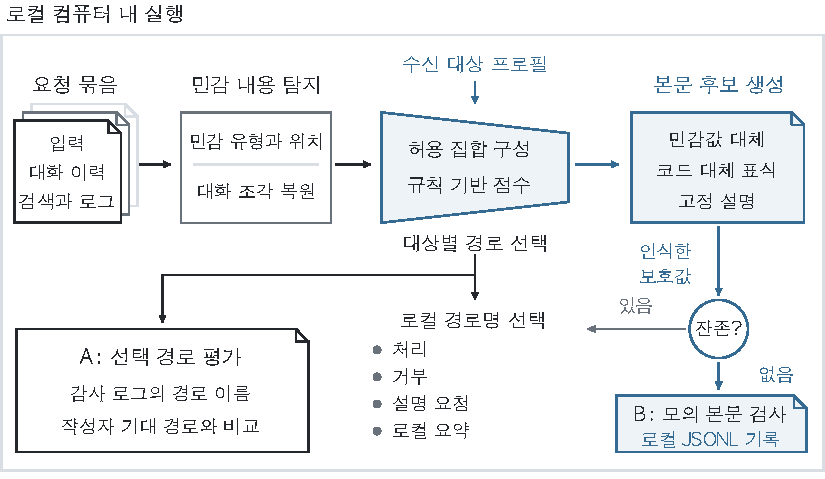
\includegraphics[width=\linewidth]{architecture-ko.pdf}
\caption{보관된 규칙 기반 구현의 실행 범위. 경로 선택 기록과 모의 전송 함수가 로컬 파일에 추가한 본문을 구분하여 점검한다. 모든 단계는 로컬에서 수행된다. 선택한 경로의 실제 업무 수행이나 외부 서버의 수신을 나타내지 않는다.}
\label{fig:architecture}
\end{figure*}
\subsection{탐지와 고정된 치환}
그림~\ref{fig:architecture}의 구현은 조립한 텍스트에서 정형 비밀값, 개인정보, 코드, 인프라와 사고 관련 단서를 검사한다. 일부 인코딩 값과 대화 조각의 결합도 지원한다. 보관된 패턴과 문맥 규칙을 사용하며 외부 탐지 제품이나 학습된 대형 분류기를 실행한 비교는 아니다.

값 가리기는 같은 개체에 일관된 대체 표식을 사용하고 원래 값과의 대응을 로컬에 남긴다. 코드 경로는 탐지한 코드 구간을 \texttt{[GENERALIZED\_CODE\_n]}으로 치환한 뒤 모든 입력에 같은 일반 설명을 덧붙인다. 입력별 알고리즘 분석, 의사코드 생성 또는 의미 보존은 구현하거나 검증하지 않았다. 경로 이름이 정책에서 의도한 충분한 변환을 달성했다는 뜻은 아니다.

\subsection{인식한 보호 값의 잔존 검사}
본문을 기록하기 전, 현재 변환 입력에서 인식한 보호 값과 코드 조각이 남는지 검사한다. 지정 검사에서 잔존이 발견되면 모의 본문을 기록하지 않고 로컬 요약 경로로 바꾼다. 구현에는 별도의 불확실 상태가 없다. 검사 결과가 비어 있으면 통과하므로, 분류 체계 밖 기밀이나 인식하지 못한 내용을 불확실하다는 이유로 차단하지 않는다.

보존한 기존 구현은 이전 대화가 있으면 최종 변환 입력을 현재 요청 문장만으로 다시 구성한다. 이전 턴은 탐지와 경로 판단에는 쓰여도 기록 본문에는 빠질 수 있다. 최초 정보 보존 점검은 이 구현을 바꾸지 않고 수행했다. 이후 별도 수정본에서는 판단에 쓴 조립 문맥 전체를 변환 입력으로 유지하고, 같은 텍스트에서 민감성 근거를 다시 구해 기존 치환과 잔존 검사를 적용했다. 정책, 탐지 규칙과 점수는 바꾸지 않았다. 수정 전후 비교는 \ref{sec:context-repair}절에 별도로 제시한다. 이는 문맥의 관련성을 골라내는 새 기능이 아니라 제공된 문맥의 일괄 삭제를 없앤 수정이다.

\subsection{모의 전송 함수가 저장하는 것}
\texttt{send\_to\_simulated\_endpoint}는 대상, 경로 관련 정보와 본문을 JSON으로 직렬화하여 로컬 JSONL 파일에 추가한다. 별도 수신 서버, 소켓 호출이나 네트워크 패킷 캡처는 없다. 보관 필드 이름에 wire가 포함되어도 실제 네트워크에서 관측한 바이트를 뜻하지 않는다.

평가에서는 경로 선택 기록과 저장된 본문을 따로 읽는다. 본문의 해시와 바이트 수를 재계산하고, 기록할 경로가 없을 때 본문 기록도 없는지 확인한다. 이는 저장 기록의 일치 점검이다. 평가 구현이나 정답 작성의 독립성, 원격 도착 또는 의미적 기밀성의 증거는 아니다.

\section{평가 방법}
\label{sec:evaluation}
\subsection{자료 구성과 비교 조건}
주 평가 SMD-Bench-1400은 기본 틀 70개에서 20개씩 변형한 합성 요청 1,400건이다. 일곱 범주에 각각 200건을 배정하였으며 로컬 대상 469건, 승인 외부 469건, 고위험 외부 462건이다. 추가 시험 SMD-Challenge-210은 핵심 결정 코드 고정 후 작성한 35개 틀의 여섯 변형이다. 스트레스 36건에는 코드 블록 속 비밀, 반복 표식과 업무상 기밀이 포함된다. 업무상 기밀 18건은 실행용 및 평가용 정책에 없는 정보 유형이다. 이 18건의 기대 경로는 사례 작성 단계에서 직접 지정하였다.

모든 비율은 고정된 합성 조건의 집계이다. 1,400건이 독립적인 실제 업무 1,400개를 대표하지 않으며 조직의 유출률을 추정하지 않는다. 추가 시험도 같은 설계자의 정책과 기대 경로를 공유한다.

여덟 비교 방식은 모두 자체 구현이다. 게이트웨이 없음, 정규식 필터와 전체 탐지 필터는 경로와 후보 문자열만 반환하고, 평가는 그 문자열을 직접 검사한다. 항상 로컬은 검사할 본문이 없다. Osaurus 방식 모사와 세 제어기 설정은 로컬 모의 기록을 남긴다. ``대상 일괄 치환'' 설정은 원래 대상을 유지한 채 대상 정보만 숨기는 실험이 아니라, 판단과 기록 모두에서 대상 프로필을 승인 외부로 바꾼다. 이 조건 차이를 대상 인식 하나의 순수한 효과로 해석하지 않는다.

전체 SMD와 경로 점수 제외 설정은 탐지, 규칙, 변환, 검사와 모의 기록을 공유하고 후보 점수 사용 여부만 다르다. 표의 Osaurus는 동작을 모사한 비교군이다. Portcullis, PRISM, Evidence-Bound와 AirGapAgent의 실제 시스템을 실행하거나 그 성능과 직접 비교하지 않았다.

\subsection{지표의 정의와 작성자 기준}
\label{sec:metrics}
\emph{경로 일치율}은 작성자가 정한 기대 경로와 선택 경로가 정확히 같은 비율이다. \emph{작성자 기준 경로 등급 미달률}은 작성자가 보안 관련으로 지정한 사례에서 외부 경로를 선택했고, 그 경로 등급이 기대 경로의 등급보다 낮은 비율이다. 등급은 값 가리기 외부=1, 코드 대체 외부=2, 네 미전송 경로=3으로 고정한다. 보안 관련 표시는 작성자 위험 유형이 있거나 원래 대상이 로컬이거나 공격 사례로 표시된 경우이다. 분모는 각 세트 전체이다.

이 등급은 평가용 순서이며 보호 효과의 실측 서열이 아니다. 지표 계산은 실제 수신자의 권한이나 허용 표현 집합을 별도로 판정하지 않는다. 따라서 0건은 독립적으로 확인한 정책 준수율이 아니다. \emph{기대한 외부 경로 미선택}은 작성자가 외부 경로를 기대했지만 미전송 경로를 고른 사례이다. 이것도 모든 합리적인 허용 기회를 기준으로 확인한 과도 차단이 아니다.

\emph{보호 값 잔존}은 후보 또는 모의 기록에 지정 값이 그대로 남는지 검사한다. \emph{표기 복원 검사}는 인코딩과 표기를 풀어 같은 값이 남는지 확인하며, \emph{코드 조각 검사}는 지정된 코드 문자열이나 구조 조각의 잔존을 검사한다. 의미를 바꾸어 공개된 사실이나 알고리즘 노출의 독립 평가는 아니다. 같은 사례가 여러 검사에 포함될 수 있다. 유형별 탐지 F1과 보관된 점수 판정 일치도 역시 작성자 표지에 따른 값이다.

\subsection{일반 실행과 작성자 유형 제공 시험}
일반 실행은 실제 탐지 규칙, 경로 선택, 본문 변환과 필요한 모의 기록을 수행한다. 별도의 \emph{작성자 유형 제공 시험}은 탐지를 생략하고 작성자가 기록한 위험 유형을 경로 결정기에 알려 준다. 내부적으로 후보 변환과 점수 계산을 할 수 있지만 경로 이름만 반환한다. 최종 기록 전 검사나 모의 전송 기록은 만들지 않는다. 스트레스 일반 실행은 36건 전체, 유형 제공 시험은 정책이 표현하지 못하는 18건을 제외한 18건이 분모이다.

원래 평가 도구는 주 평가 60건에서 공격 유형 표지를 읽어 다중 턴 민감성 표시를 미리 넣었다. 후속 비교는 보관 코드의 두 복사본 중 하나에서 이 표시를 넣는 두 줄만 제거하였다. 세 세트의 같은 입력 1,646건을 모두 다시 실행했고 실제 대화, 탐지기, 정책, 기대 경로와 채점은 유지하였다. 추가 시험과 스트레스에는 원래 이 표시가 없었다. 모델 능력 가정을 포함한 다른 부가 정보도 유지했으므로 모든 평가용 정보의 영향을 제거한 실험은 아니다.

\begin{figure*}[tbp]
\centering
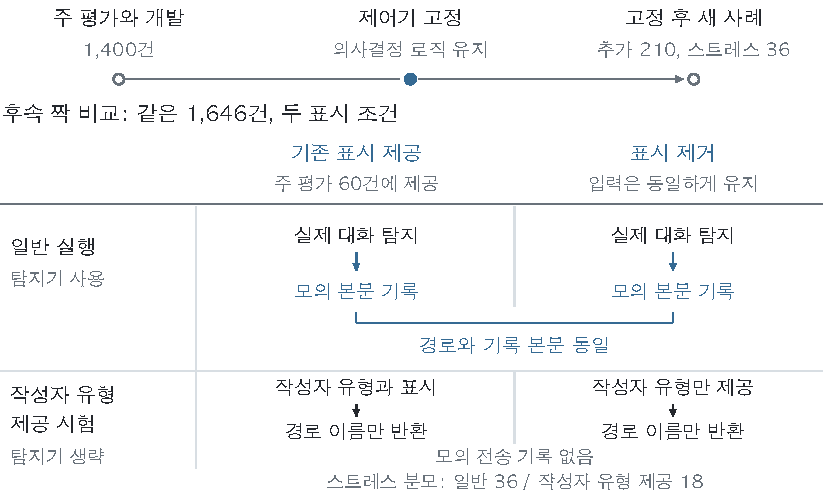
\includegraphics[width=\linewidth]{protocol-ko.pdf}
\caption{평가용 표시 제거의 짝지은 비교. 같은 1,646건을 원래 조건과 표시 제거 조건에서 점검한다. 일반 실행은 탐지와 모의 기록을 수행하고, 작성자 유형 제공 시험은 탐지를 생략하여 경로만 반환한다. 아래의 별도 정보 보존 자료와 새 검토 후보는 이 1,646건에 포함되지 않는다.}
\label{fig:protocol}
\end{figure*}

\subsection{이전 대화의 업무 정보 보존 점검}
기존 구조 참고 파일럿은 자동 분류한 업무 유형과 문맥 단서만으로 새로 지은 15개 과제를 세 대상 조건에 적용한 45건이다. 민감성, 대상 조건과 기대 경로는 연구자가 추가했다. 제어기와 정책은 과제 작성 전에 고정했고, 기대 경로나 검사용 보호 값 목록을 별도 정답 채널로 주지 않았다. 보호할 가상 값 자체는 요청에 포함된다.

두 설정을 각각 45건 실행하였다. 외부 기록 금지에 대한 연구자 가설은 23건, 조건부 허용은 20건, 첨부 부재로 미확정은 2건이다. 네 과제는 이전 턴이 있으며 검색 자료나 로그를 넣은 과제는 없다. 지정 업무 숫자나 단어가 모의 본문에 남았는지를 실제 기록이 있고 지정 값도 있는 조건에서만 확인한다. 이는 응답 품질이나 원문 업무의 대표성을 측정하는 시험이 아니다. 15과제와 세 대상 변형은 여덟 생성 범주를 공유하므로 독립인 45개 업무로 보지 않는다.

\subsection{원문 업무 구조를 반영한 후속 검토 자료}
기존 파일럿의 거친 유형 분류를 보완하기 위해, 같은 선택 그룹에서 실무 프롬프트 원문 창 15개를 기기 내 언어 모델로 읽어 업무 단계의 순서, 요구 산출물과 문맥 의존성을 고정된 분류값으로 기록하였다. 원문을 외부 모델에 보내거나 원문 표현을 산출물에 복사하지 않았다. 이 분류는 사람의 원래 의도를 확인한 정답이 아니라 원문을 참고한 모델 보조 구조 코딩이다.

원문 창의 잘림, 필요한 앞 대화 또는 첨부 부재 때문에 7개를 보류하고 8개 구조만 새 합성 과제로 만들었다. 모델이 분류한 단계 순서와 산출물을 참고하되 사실, 인물, 수치, 코드와 자료는 새로 만들었다. 실제 도구 환경도 가상 자료로 대체하였다. 민감성과 세 대상 조건은 연구자가 추가한 실험 조건이다. 새 8과제와 대상별 24조건은 두 검토자용 자료로 준비했으며 실행하지 않았다. 기존 45조건의 결과를 이 자료의 성능으로 옮기지 않는다. 원문 선별과 실제 구조 코딩의 범위는 부록~\ref{app:d64}에 제시한다.

\subsection{실제 로컬 모델과 HTTP 경로의 별도 비교}
\label{sec:live-method}
기존 규칙 기반 실험과 별도로, aethon 앱의 \texttt{smd\_app.engine.execute}를 직접 호출하는 평가 실행기를 구성했다. 이 백엔드는 보관된 \texttt{process\_request}의 직접 재실행이 아니라 앱의 후속 구현이다. 새 정책과 경로를 과거 정답으로 채점하지 않으며 기존 수치를 이 모델의 성능으로 옮기지 않는다. 앱과 평가 실행기는 같은 정책 집행, 패턴 검사, 본문 변환, 최종 보호 값 검사와 모델·제공자 어댑터를 사용한다. 실행기만의 축약된 게이트웨이로 앱의 성능을 대신하지 않는다. 다만 평가의 진입점은 데스크톱 화면이 아니라 백엔드 함수이며, 검색·첨부·도구 결과는 지원되는 텍스트 메시지에 붙인 합성 추출문이다. 이 비교로 실제 검색, 바이너리 첨부 추출이나 운영체제 도구 실행을 평가했다고 주장하지 않는다.

새 자료는 수치·표 계산, 사실 추출, 코드·알고리즘, 문맥 완전성의 네 범주에 세 과제씩 배정한 12개 작성자 생성 과제이다. 네 과제는 이전 턴을 필요로 한다. 각 과제의 순서 있는 전체 메시지는 그대로 두고 로컬, 승인 외부, 제한 외부의 세 프로필만 바꾼다. 따라서 36조건은 독립 업무 36개가 아니다. 한 장비의 실제 추론으로 정확한 값 검사를 수행하기 위한 소규모 범주 배분이며 통계적 검정력으로 정한 크기가 아니다. 기존 45조건 및 준비된 24조건은 이 자료에서 제외했고, 새 40과제·120조건 계획을 완료한 것으로 세지 않는다. 실제 업무 원문의 표현, 사실, 수치와 코드를 재사용하지 않았으며 실무 자료의 분포나 의도를 독립적으로 재현한 표본도 아니다.

모델은 Qwen 팀의 공개 가중치 \texttt{Qwen3-4B}~\citep{qwen}를 Ollama 배포 \texttt{qwen3:4b}로 실행한다. 표~\ref{tab:live-model-config}에 설치한 파일과 설정을 명시한다. 상류 학습 체크포인트의 revision은 설치 패키지에서 확인하지 못했으므로 현재 상류 HEAD로 대신하지 않는다. 설치한 양자화 가중치·템플릿·설치 정보 목록(manifest)의 해시가 이번 실행 대상을 식별한다. 자연어 정책 해석은 주 비교의 매 사례에서 다시 수행하지 않고, 연구자가 작성한 실행 정책을 프로그램 스키마로 검증한 뒤 한 번 고정한다. 정책 작성은 AI가 보조했으며 조직 보안 책임자나 두 독립 검토자의 승인·판정은 아니다. 자연어 문장 여섯 개의 해석 점검은 별도 진단으로 분리한다.

\begin{table*}[tbp]
\centering
\caption{새 로컬 모델 비교의 고정 조건. 해시 전체와 시스템 지침·채팅 템플릿·구조화 출력 형식은 실행 명세에 보관한다. 평가한 한 모델을 모든 공개 가중치 모델의 대표로 보지 않는다.}
\label{tab:live-model-config}
\smalltable
\begin{tabular}{@{}p{.26\linewidth}p{.69\linewidth}@{}}
\toprule
항목 & 실행 조건 \\
\midrule
모델과 라이선스 & Qwen3-4B, GGUF Q4\_K\_M, Apache-2.0 공개 가중치. 학습 자료 전체의 공개성은 미확인. \\
가중치 식별 & SHA-256 시작 \texttt{3e4cb14174460404}, 2,497,280,480바이트. \\
실행 환경 & Ollama 0.40.13, Python 3.12.13, Apple M4, 통합 메모리 16 GiB, macOS 27.2. \\
문맥·출력 한도 & 일반 문맥 8,192; 큰 구조 검사 분기 32,768. 검사 출력 최대 4,096, 업무 답변 최대 2,048토큰. \\
생성·재실행 & 무작위성 설정 temperature=0 요청, 난수 시작값(seed) 고정은 앱에서 미지원, think=false 요청. 자동 재시도 0회. \\
제한 시간 & 한 조건 240초, 로컬 추론 HTTP 180초(연결 3초), 제공자 HTTP 240초(연결 10초). 리다이렉트 없음. \\
대화 상태 & 매 회 명시한 새 메시지 목록. 이전 답변 재사용 없음. 가중치와 엔진의 공통 입력 캐시는 유지될 수 있음. \\
\bottomrule
\end{tabular}
\end{table*}

비교 조건 A는 로컬 전용이다. B는 앱의 결정적 패턴 검사와 고정된 검사 응답을 사용하고 실제 모델로 업무를 수행한다. 그 고정 응답은 추가 의미적 발견이 없고 불확실하지 않으며 로컬 처리가 부족하다는 선호를 제공한다. A도 같은 고정 응답을 사용하되 목적지를 로컬로 고정한다. 패턴에 따른 기존 발견과 공통 거부·설명 요청 통제는 남긴다. C는 같은 로컬 모델이 전체 문맥을 구조화된 형식으로 검사하여 추가 민감성 근거와 로컬 처리 가능성을 제안한다. 이 가능성은 모델의 추정이며, 먼저 완성 답안을 생성하여 실제 성공을 확인한 결과가 아니다. C의 검사가 실패하거나 확실하지 않으면 외부 위임을 제한한다. 모델은 실행 정책을 고치거나 외부 권한을 만들지 않는다. B와 C는 의미 검사, 불확실성 및 처리 가능성 입력을 함께 바꾸므로 각 요인의 독립적인 효과를 분리한 비교가 아니다.

승인 외부 조건은 앱의 기본 실행 정책에서 자격증명, 개인정보, 사내 인프라와 코드를 외부 전송 전에 가리고 업무상 기밀 및 미확인 유형은 로컬에 두도록 한다. 제한 외부 조건은 같은 제약에 ``모든 요청을 로컬에 둔다''는 R8을 추가하고 충돌하는 일반 허용 규칙 R7에서 해당 외부 목적지를 뺀다. 모든 비교군은 동일한 대상별 정책을 사용한다. 승인이라는 이름은 합성 자료의 가상 권한이며 특정 실제 공급자의 계약 상태를 뜻하지 않는다.

\begin{figure*}[tbp]
\centering
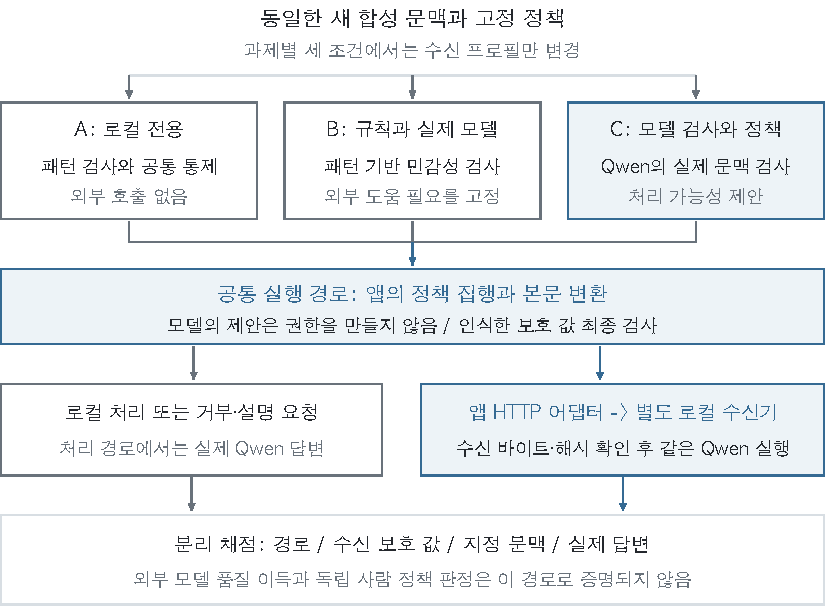
\includegraphics[width=\linewidth]{live-model-ko.pdf}
\caption{새 모델 비교의 실행 및 관측 경로. 외부 경로의 HTTP 요청은 별도 로컬 수신기가 받고, 변환된 메시지를 같은 Qwen 모델로 처리한다. 따라서 실제 바이트 수신과 변환의 영향을 확인할 수 있으나 더 강한 외부 모델의 업무상 이득은 측정하지 않는다.}
\label{fig:live-model}
\end{figure*}

외부 경로는 앱의 실제 \texttt{ProviderRegistry.complete} HTTP 어댑터를 통과하여 별도 loopback 수신 프로세스에 보낸다. 이 수신기는 받은 원시 바이트의 길이와 SHA-256을 파싱 전에 독립 계산한다. 어댑터가 직렬화한 요청의 바이트 일치와, 화면 전송 표시의 입력인 변환 이벤트 메시지와 수신 JSON의 일치를 따로 검사한다. 이것만으로 모든 실행을 데스크톱 화면에서 직접 관찰했다고 주장하지 않는다. 수신기는 받은 문맥을 같은 Qwen의 \texttt{LocalRuntimes.chat}으로 처리하고 OpenAI 호환 응답을 반환한다. A의 로컬 답변과 B·C의 로컬 및 HTTP 경로 답변은 같은 모델과 답변 한도를 사용한다. 이는 실제 HTTP 통신을 포함한 통제 실험이며 실제 외부 제공자나 더 강한 모델의 응답 품질 실험이 아니다.

실행 전에 코드·정책·모델 설정·입력·그룹·보호 값·업무 성공 기준과 빈 검토자 자료의 해시를 고정한다. 과제별 세 수신 조건과 A·B·C를 한 번씩 실행한 108회에 대해 실패, 시간 초과와 형식 오류도 남기고 성공 출력만 고르지 않는다. Qwen에 think=false를 요청해도 추론 구분자가 관찰될 수 있으므로 추론 계산이 전혀 없다고 가정하지 않는다. 보고된 생성 토큰을 남기고 최종 답변을 채점한다. 평범한 데스크톱 프로세스가 함께 실행되는 장비의 지연이므로 독점 자원 성능으로 일반화하지 않는다.

과제와 업무 기준은 연구자 정의이며 생성형 AI가 작성을 보조했다. 업무 채점은 사전에 계산한 JSON 필드의 숫자 또는 공백·대소문자를 정규화한 문자열과 비교한다. 코드 블록이나 주변 문장 속 JSON도 허용하며 추가 필드는 오답으로 보지 않는다. 요청된 첨부가 없는 과제는 사실을 지어내는 대신 지정한 미해결 상태를 답해야 한다. 이 좁은 실행 검사는 실제 생성 답변의 정해진 값을 측정하지만 독립 사람의 전반적 품질 판정은 아니다. 보호 값의 직접·표기 복원·코드 조각 잔존, 지정 문맥의 문자열 보존과 답변 채점은 따로 집계한다. 두 검토자에게는 전체 합성 문맥, 대상과 자연어 정책만 주도록 별도 묶음을 준비하고 허용 집합, 선호 경로, 정책 근거와 불확실성을 각각 빈 답변란에 남겼다. 사람 답변이 없으므로 이 비교는 사람 허용 집합 준수나 사람 선호 일치를 측정하지 않는다.

\subsection{실제 제공자의 고정 표현 추가 진단}
\label{sec:external-method}
주 비교 108회를 모두 마친 뒤, 실제 제공자에 보낼 수 있는 고정 표현을 대상으로 별도 진단을 구성했다. B의 승인 외부 조건에서 이미 선택·변환되고 loopback 수신까지 확인된 본문을 후보로 삼았다. 연구자 검사 기준의 직접·표기 복원 보호 값이나 코드 조각이 남는 두 본문을 추가 안전 검사로 제외하고 열 본문을 고정했다. 원래 Qwen 답변의 성공 여부는 선택 기준이 아니었다. 이 선별은 주 비교 결과를 확인한 뒤 수행한 연구자 통제이며, 일반 앱이나 C가 실제 제공자 앞에서 이 두 본문을 차단했다고 집계하지 않는다. 새로운 독립 업무나 40과제 시험으로도 세지 않는다.

외부 모델은 요청 식별자 \texttt{gpt-5.4-mini-2026-03-17}로 고정했다~\citep{openaimodel}. 모델은 업무 답변만 생성하며 민감성 검사나 경로 선택, 정책 해석에 참여하지 않는다. 앱의 \texttt{provider\_agent\_complete} 어댑터로 공식 \texttt{/v1/chat/completions}에 같은 고정 메시지를 보냈다. temperature=0, reasoning\_effort=none, 출력 한도 2,048, stream=false, store=false, 시간 한도 120초, 재시도 0회이며 seed는 지정하지 않았다. API 내부 가중치와 채팅 템플릿은 확인할 수 없으며 요청한 모델 식별자와 응답 모델·설정을 기록한다. 앞선 loopback 조건의 같은 Qwen 실행과 구분한다.

이 진단은 \texttt{engine.execute}의 A·B·C를 다시 실행하지 않고 이미 고정한 표현의 외부 답변만 확인한다. C의 로컬 선호를 외부 위임으로 바꾸거나 실행 정책을 약화하지 않았다. 실제 데스크톱 Quick Chat의 OpenAI 연결은 별도의 Responses API 경로이므로, 이 결과를 GUI에서 실제 외부 위임까지 완료한 검증으로 부르지 않는다.

클라이언트가 직렬화한 요청 바이트·해시, 제공자 응답과 요청 ID, 토큰 사용량을 남긴다. 실제 제공자에서 수신 본문을 독립 관측한 증거는 없다. 앞선 loopback은 별도 기기 내 수신기가 직접 받은 바이트를 계산한 조건이며, 이 진단의 클라이언트 송신 관측과 구분한다. 성공 응답과 store=false만으로 제공자의 보관·재학습 조건이나 금지 의미의 부재를 검증하지 않는다. 공개 요율의 비캐시 입력과 출력 단가를 보고된 사용량에 적용한 비용 상한은 실제 청구서와 구분한다.

\section{결과}
\label{sec:results}
\subsection{경로 등급과 보호 값 잔존의 차이}
\begin{table*}[tbp]
\centering
\caption{주 평가 70개 틀, 1,400조건의 자체 비교 결과. 세 비율의 분모는 모두 1,400이다. 경로 일치와 등급 미달은 작성자 기준이다. 본문 검사 대상의 후보는 생성한 문자열, 기록은 로컬 모의 파일을 뜻한다. 없음은 미전송으로 검사할 본문이 없다는 뜻이다.}
\label{tab:baseline}
\footnotesize\setlength{\tabcolsep}{2pt}\renewcommand{\arraystretch}{1.15}
\begin{tabular*}{\linewidth}{@{\extracolsep{\fill}}llrrrr@{}}
\toprule
비교 설정 & 검사 대상 & \shortstack{경로\\일치율} & \shortstack{등급\\미달률} & \shortstack{외부 경로\\미선택률} & \shortstack{보호 값\\잔존(건)} \\
\midrule
게이트웨이 없음 & 후보 & 34.21\% & 64.86\% & 0.00\% & 880 \\
항상 로컬 & 없음 & 37.86\% & 0.00\% & 37.50\% & 0 \\
정규식 필터 & 후보 & 34.21\% & 64.86\% & 0.00\% & 240 \\
전체 탐지 필터 & 후보 & 34.21\% & 64.86\% & 0.00\% & 0 \\
Osaurus 방식 모사 & 기록 & 34.21\% & 64.86\% & 0.00\% & 0 \\
대상 일괄 치환 & 기록 & 63.50\% & 21.50\% & 5.14\% & 0 \\
경로 점수 제외 & 기록 & 98.36\% & 0.00\% & 0.00\% & 0 \\
전체 SMD & 기록 & 94.14\% & 0.00\% & 5.14\% & 0 \\
\bottomrule
\end{tabular*}
\par\smallskip
\parbox{\linewidth}{\footnotesize 대상 일괄 치환은 판단과 기록 대상 모두 승인 외부로 바꾼 설정이다. 미전송의 잔존 0건은 업무 수행이나 안전성이 검증되었다는 뜻이 아니다.}
\end{table*}
RQ1에서 게이트웨이 없음, 정규식 필터와 전체 탐지 필터의 후보 문자열에 남은 보호 값은 각각 880건, 240건, 0건이지만 경로 등급 미달률은 모두 64.86\%였다(표~\ref{tab:baseline}). 값 제거와 작성자가 정한 경로 순서는 서로 다른 지표이기 때문이다. 이 수치만으로 실제 수신 권한 위반율을 구할 수는 없다.

전체 SMD는 등급 미달 0건, 기대 경로 일치 1,318/1,400건(94.14\%)이었다. 외부 경로를 기대한 72건은 미전송 경로를 선택했다. 항상 로컬의 해당 미선택률은 전체 조건의 37.50\%였다. 기록을 남기지 않은 결과와 허용된 작업을 적절히 수행한 결과를 같은 성공으로 합치지 않는다. 그림~\ref{fig:baseline}은 여섯 설정의 두 경로 지표를 같은 축에서 비교한다.

\begin{figure*}[tbp]
\centering
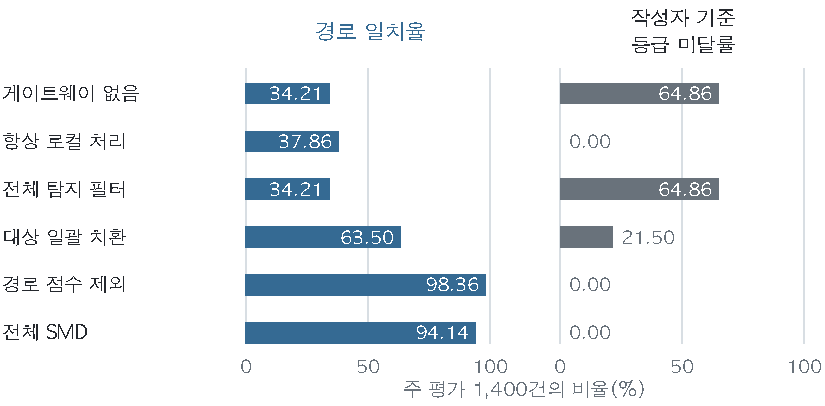
\includegraphics[width=\linewidth]{baseline-ko.pdf}
\caption{주 평가의 두 경로 지표. 경로 일치는 기대 경로와의 정확한 일치이며 등급 미달은 작성자 순서에 따른 대리 지표이다. 후자가 0\%여도 실제 대상 권한과 표현의 적절성이 검증된 것은 아니다. 여덟 설정 전체는 표~\ref{tab:baseline}에 제시하였다.}
\label{fig:baseline}
\end{figure*}

\subsection{점수와 평가용 표시의 영향}
\begin{table*}[tbp]
\centering
\caption{기존 합성 자료와 표시 제거 비교의 결과. 주 평가 70개 틀, 추가 시험 35개 틀과 별도 스트레스 조건의 집계이다. 일반 실행은 두 표시 조건에서 같아 한 번만 적고 유형 제공 시험은 조건을 나눈다. 모든 일치는 작성자 기대 경로 기준이다.}
\label{tab:datasets}
\smalltable
\begin{tabular*}{\linewidth}{@{\extracolsep{\fill}}lrrr@{}}
\toprule
측정 항목 & 주 평가 & 추가 시험 & 스트레스$^{a}$ \\
\midrule
일반 실행 조건 수 & 1,400 & 210 & 36 \\
모의 본문 기록 수 & 453 & 53 & 16 \\
일반 실행 경로 일치 & 94.14\% & 87.62\% & 66.67\% \\
유형 제공: 원래 표시$^{b}$ & \shortstack{1,395/1,400\\(99.64\%)} & \shortstack{192/210\\(91.43\%)} & 18/18 \\
유형 제공: 표시 제거$^{b}$ & \shortstack{1,369/1,400\\(97.79\%)} & \shortstack{192/210\\(91.43\%)} & 18/18 \\
작성자 기준 등급 미달 & 0 & 0 & 8 \\
기대한 외부 경로 미선택 & 72 & 18 & 0 \\
보호 값 직접 잔존 & 0 & 0 & 8 \\
표기 복원 후 잔존 & 0 & 0 & 8 \\
지정 코드 조각 잔존 & 0 & 0 & 0 \\
유형별 탐지(매크로 F1) & 93.55\% & 86.72\% & 85.71\% \\
규칙 기반 점수 판정 일치 & 91.50\% & 89.52\% & 88.89\% \\
\bottomrule
\end{tabular*}
\par\smallskip
\parbox{\linewidth}{\footnotesize $^{a}$스트레스 일반 실행은 36건 전체이다. 유형 제공 시험은 정책에 없는 업무상 기밀 18건을 제외한 18건이며 제외된 조건에 기밀 잔존 8건이 모두 포함된다. 같은 사례가 여러 잔존 검사에 중복 집계될 수 있다.\par
$^{b}$원래 표시 조건은 주 평가 60건에 공격 유형 표지로부터 민감성 표시를 제공한다. 제거 조건은 이 경로만 없애고 실제 대화 탐지기는 유지한다. 두 조건 모두 세 자료를 전부 재실행했다. 유형 제공 시험은 내부 후보 변환을 할 수 있으나 최종 기록 전 검사나 모의 기록을 하지 않는다.}
\end{table*}
RQ2에서 경로 점수를 끄자 주 평가 일치율은 94.14\%에서 98.36\%로 높아졌다. 기본 점수가 작성자 선호 경로를 더 잘 고른다는 근거는 없다. 가중치 분석의 일치율 범위는 주 평가 74.43--99.07\%, 추가 시험 73.33--93.33\%였으며 실제 업무 성공률이 아니다.

표~\ref{tab:datasets}의 표시 제거 비교에서는 세 자료 모두 일반 실행의 경로, 등급 지표와 지정 값 잔존 결과가 같았다. 탐지기가 원래 표시 대상 60건의 실제 대화에서 단서를 다시 찾았기 때문이다. 각 조건의 모의 기록 $453+53+16=522$건을 다시 읽어 비교한 대상과 본문도 같았다. 이는 로컬 저장 기록의 동일성이고 원격 도착을 검증한 결과가 아니다.

탐지를 생략한 유형 제공 시험에서는 주 평가 26건이 로컬 요약에서 값 가리기 외부 경로로 바뀌었다. 기대 경로 일치는 1,395/1,400건(99.64\%)에서 1,369/1,400건(97.79\%)으로 변했다. 서로 다른 입력 조건의 차이는 $100\times26/1{,}400=1.857\ldots$, 즉 1.86\%포인트이다. 이 시험은 경로 이름만 반환하므로 추가 모의 전송이나 실제 유출이 발생한 것은 아니다. 추가 시험 192/210건과 스트레스 18/18건은 유지되었다. 실제 대화에서 복원한 표시를 넣어 원래 주 평가 선택을 복구한 보조 점검은 이 주 비교와 구분한다. 미지 요청이나 모든 부가 정보 의존성에 일반화하지 않는다.

\subsection{분류 체계 밖 기밀의 잔존}
추가 시험 경로 일치는 184/210건(87.62\%), 스트레스는 24/36건(66.67\%)이었다. 스트레스의 업무상 기밀은 모의 본문 8건에 남았고 직접 검사와 표기 복원 검사 모두에서 확인되었다. 이는 같은 8건에 대한 결과이며 서로 다른 16건이 아니다. 해당 유형이 실행용과 평가용 정책에 없으므로 경로 제한과 인식한 값의 검사로는 제거하지 못했다.

정책이 표현하는 18건에서 작성자 유형을 주어 18/18건 일치한 결과는 제외된 기밀 사례에 대한 해결책을 검증하지 않는다. RQ3의 첫 관찰은 규칙에 따른 선택과 그 규칙이 내용의 기밀성을 충분히 표현하는지가 다른 문제라는 점이다.

\subsection{이전 턴의 지정 정보 누락}
\begin{table*}[tbp]
\centering
\caption{수정 전 구현의 기존 구조 참고 합성 파일럿: 15과제, 설정별 45조건. 연구자 가설과 비교한 탐색적 집계이며 독립 사람 정답이나 원래 실무의 성능이 아니다. 기존 1,400건 및 후속 준비 후보와 합산하지 않는다.}
\label{tab:pilot}
\smalltable
\begin{tabular*}{\linewidth}{@{\extracolsep{\fill}}lrr@{}}
\toprule
측정 항목 & 전체 SMD & 점수 제외 \\
\midrule
연구자 선호 경로와 일치 & 44/45 & 42/45 \\
연구자가 금지로 정한 조건의 기록 & 0/23 & 0/23 \\
외부 경로 기대 조건의 미선택 & 1/20 & 1/20 \\
모의 본문 기록 수 & 19 & 21 \\
보호 값 잔존(직접 및 표기 복원) & 0/19 & 0/21 \\
지정 코드 조각 잔존 & 0/19 & 0/21 \\
지정 업무 정보 누락$^{a}$ & 6/18 & 6/18 \\
\bottomrule
\end{tabular*}
\par\smallskip
\parbox{\linewidth}{\footnotesize $^{a}$분모는 지정 정보가 있고 모의 기록도 있는 18조건이다. 미기록은 각각 26건과 24건이다. 누락 6건은 세 과제의 두 대상 변형으로 독립인 여섯 업무가 아니다. 문자열 잔존의 보조 검사이며 실제 답변 품질이 아니다.}
\end{table*}
표~\ref{tab:pilot}의 공통 모의 기록 19건은 본문이 같다. 점수 제외 설정의 추가 기록 2건은 참조 그림이 없다고 명시한 과제의 두 외부 조건이다. 전체 SMD는 추가 설명 요청을 선택했다. 두 조건의 외부 허용 여부는 사전에 미확정으로 두었으므로 확정된 정책 위반이나 안전한 선택으로 집계하지 않는다. 코드와 개인정보가 함께 있는 한 조건은 연구자 선호와 달리 두 설정 모두 로컬 요약을 골랐다. 이는 유형별 경로 교차 적용과 대체 규칙의 결과이며 점수 효과나 독립적으로 확인한 과도 차단이 아니다.

양쪽 모두 지정 업무 정보가 있는 모의 본문 18건 중 6건에서 해당 정보가 빠졌다. 세 과제의 두 외부 조건이며, 빠진 숫자나 단어는 모두 이전 턴에만 있었다. 이전 대화가 있으면 현재 요청만으로 최종 본문을 다시 구성하는 동작이 직접 원인이다. 경로 판단에 사용한 문맥이 기록 본문에는 없을 수 있다. 다만 이것이 외부 응답 실패를 뜻하는지는 품질 평가가 필요하다. 44/45와 42/45의 연구자 선호 일치 차이로 점수 설정의 우수성을 주장하지 않는다.

\subsection{문맥 보존 수정과 전후 비교}
\label{sec:context-repair}
기존 구현과 실행 결과를 보존한 뒤 별도 코드 복사본에서 최종 변환 입력만 수정했다. 현재 요청만 남기는 대신 이전 턴과 검색 자료·로그를 포함한 조립 문맥을 유지하고, 그 문맥에서 탐지한 보호 값을 기존 방식으로 치환·검사한다. 이미 누락을 발견한 같은 45조건을 두 구현과 두 점수 설정으로 다시 실행했으므로, 이 비교는 알려진 결함의 회귀 점검이며 독립적인 새 성능 시험이 아니다. 기대 경로와 보호 값·업무 정보 기준은 바꾸지 않았다. 실행은 모두 로컬 모의 기록이며 네트워크 수신 관측이 아니다.

\begin{table*}[tbp]
\centering
\caption{같은 45조건의 문맥 보존 수정 전후. 괄호나 분수의 분모는 해당 지표의 관측 단위이며, 사람 판정이나 실제 답변 품질을 뜻하지 않는다.}
\label{tab:context-repair}
\smalltable
\begin{tabular*}{\linewidth}{@{\extracolsep{\fill}}lrrrr@{}}
\toprule
 & \multicolumn{2}{c}{전체 SMD} & \multicolumn{2}{c}{점수 제외} \\
측정 항목 & 수정 전 & 수정 후 & 수정 전 & 수정 후 \\
\midrule
지정 업무 정보 누락 & 6/18 & 0/18 & 6/18 & 0/18 \\
모의 본문 기록 수 & 19 & 19 & 21 & 21 \\
연구자 금지 조건의 기록 & 0/23 & 0/23 & 0/23 & 0/23 \\
보호 값 직접 잔존 & 0/19 & 0/19 & 0/21 & 0/21 \\
표기 복원 후 보호 값 잔존 & 0/19 & 0/19 & 0/21 & 0/21 \\
지정 코드 조각 잔존 & 0/19 & 0/19 & 0/21 & 0/21 \\
\bottomrule
\end{tabular*}
\end{table*}

표~\ref{tab:context-repair}에서 양쪽 설정 모두 누락 6/18조건이 0/18조건으로 줄었다. 세 과제의 두 외부 대상 조건에서 지정한 숫자와 단어가 모두 모의 본문에 남았고, 보호 값과 코드의 지정 잔존 검사는 증가하지 않았다. 경로와 기록 수는 같고 설정별 본문 6건이 달라졌다. 이는 필요한 것으로 지정한 문자열의 회복이며, 모든 업무 문맥의 충분성이나 최소 공개, 의미적 기밀성 또는 답변 품질을 입증하지 않는다.

기존 1,400건·210건·36건도 두 구현과 두 설정으로 비교했다. 파일럿을 포함한 1,691입력의 설정별 비교, 총 3,382쌍에서 경로는 모두 같았다. 주 평가 모의 본문은 설정별 13건이 바뀌었으나 보호 값 잔존은 0건으로 유지됐다. 추가 시험의 본문은 같고 잔존 0건, 스트레스 본문도 같고 기존 업무상 기밀 잔존 8건이 유지됐다. 코드 조각 잔존도 증가하지 않았다. 따라서 앞 절의 평가용 표시 제거에서 본문이 같았다는 결과와, 이번 문맥 보존 수정에서 일부 본문이 바뀐 결과를 구분해야 한다. 과거 집계 표의 수치를 새 구현 결과로 덮어쓰지 않았다.

추가로 과거 턴의 비밀값, 개인정보·인프라와 검색 자료·로그의 결합, 턴에 나뉜 비밀값, 비공개 코드, 사고 문맥, 숨은 지침 추출을 다루는 새 합성 회귀 과제 6개를 세 대상과 두 설정에 적용했다. 구현별 36회 실행에서 모의 기록은 8건으로 같고 지정 보호 값 잔존은 0건이었다. 원래 빠졌던 공개 업무 정보는 6회에서 0회로 줄었으며, 로컬 전용·분할 비밀·사고·숨은 지침 및 고위험 대상 코드 조건의 미기록은 유지됐다. 이는 수정 후 작성한 진단 점검이며 독립적인 표본이나 사람 검토로 집계하지 않는다.

\subsection{실제 모델의 업무 검사와 수신 본문}
\label{sec:live-results}
RQ4의 새 비교는 12개 작성자 생성 과제를 세 수신 조건과 A·B·C에서 한 번씩 실행한 108회이다. 고정한 입력·정책·검사 기준과 백엔드 해시는 실행 뒤에도 같았다. 모든 실패를 남겼고 표~\ref{tab:live-results}의 업무 검사 분모는 각 군의 36조건이다. 이는 Qwen을 사용하지 않은 앞 절의 1,400건·210건·36건 결과와 합산하거나 직접 같은 정확도로 비교하지 않는다.

\begin{table*}[tbp]
\centering
\caption{Qwen3-4B의 새 12과제·36수신 조건 비교. A는 로컬 전용, B는 결정적 검사·외부 선호, C는 실제 모델 검사와 고정 정책이다. 세 대상 조건은 같은 과제의 반복이며 독립 업무 36개가 아니다. 대시는 HTTP 수신이 없어 측정할 수 없음을 뜻한다.}
\label{tab:live-results}
\smalltable
\begin{tabular*}{\linewidth}{@{\extracolsep{\fill}}lrrr@{}}
\toprule
측정 항목 & A & B & C \\
\midrule
실행 조건 수 & 36 & 36 & 36 \\
사전 지정 응답 필드 검사 통과 & 36/36 & 32/36 & 34/36 \\
실행 실패: 생성 한도 도달 & 0 & 3 & 2 \\
실제 loopback HTTP 수신 & 0 & 12 & 0 \\
수신 바이트·변환 메시지 일치 & -- & 12/12 & -- \\
직접·표기 복원 보호 값 잔존 & -- & 2/12 & -- \\
지정 코드 조각 잔존 & -- & 0/12 & -- \\
지정 업무 정보 누락 & -- & 0/10 & -- \\
실제 로컬 모델 호출 & 36 & 36 & 72 \\
백엔드 지연 중앙값(초) & 17.26 & 19.75 & 24.14 \\
\bottomrule
\end{tabular*}
\par\smallskip
\parbox{\linewidth}{\footnotesize 보호 값은 다섯 값이 남은 두 본문이다. 다섯 건의 실패도 36조건에 포함한다. 특히 B의 실패 두 건은 HTTP 수신 뒤 답변 생성이 한도에 도달했으므로 수신·잔존 검사 분모 12에서 빼지 않는다. 지정 업무 정보는 해당 검사가 가능한 수신 본문 10건이 분모이다. A·C의 수신 보호는 0건의 안전 성공이 아니라 미측정이다. 지연은 백엔드 execute 호출부터 반환·실패까지이며 런타임 시작, 모델 다운로드, GUI와 사람 입력 시간을 제외한다.}
\end{table*}

로컬 및 제한 외부 프로필의 24조건에서는 세 군 모두 외부 HTTP 호출이 없었다. 그러나 승인 외부라는 대상 조건을 만족한 B의 수신 본문 2/12건에는 지정 보호 값이 남았다. 이는 허용된 대상에 보냈다는 사실과 허용된 정보 표현만 보냈다는 사실을 구분해야 함을 보여 준다. 직접 및 표기 복원 검사가 같은 두 본문을 찾았고, 지정 코드 조각 검사는 0/12건이었다. 지정 정보가 있는 10건의 필요한 문자열은 모두 남았으나, 그 사실만으로 보호·업무 성공을 함께 판정하지 않는다.

C의 36회 모두 모델은 로컬 처리가 충분하다고 제안했고, 최종 정책 프로그램은 로컬 처리 18회와 로컬 요약 18회를 선택했다. 검사 결과 중 근거를 갖춘 신뢰 가능한 결과로 수용한 것은 25/36건이며, 나머지 11건은 외부 위임을 제한하는 대체 처리로 이어졌다. 이는 단순히 유효 JSON이 25건이라는 수치나 사람 판정 정확도가 아니다. C는 주 비교에서 외부 경로를 한 번도 선택하지 않았으므로 C의 외부 본문 변환 성능을 측정했다고 할 수 없다. 같은 36조건에서 A만 통과하고 B가 통과하지 못한 경우는 4건, A만 통과하고 C가 통과하지 못한 경우는 2건이었다. B와 C는 31건에서 함께 통과했고 B만 통과 1건, C만 통과 3건, 둘 다 미통과 1건이었다. 이 자료는 C가 로컬 전용보다 업무 검사를 개선했다는 근거가 아니다.

실패 다섯 건은 모두 네이티브 추론의 출력 한도 도달로 남았으며 B의 완료 답변 한 건도 사전 필드 값 검사를 통과하지 못했다. 자동 재시도나 성공 출력 선택은 없었다. 전체 지연 평균은 A 20.59초, B 24.29초, C 29.13초이고, C의 검사 단계 중앙값은 6.24초였다. 실제 추론 호출은 각각 36, 36, 72회이며 준비 확인 호출은 별도이다. 네이티브 요청에서 다시 계산한 입력/생성 토큰은 A 4,626/24,174, B 4,852/28,490, C 24,471/33,960이다. 생성 한도 실패의 계산도 포함한다. 입력·출력과 캐시 상태가 다르므로 전체 지연 차이를 검사 한 요인의 순수 비용으로 해석하지 않는다. 이 주 비교의 실제 외부 제공자 호출과 추론 요금은 0이며 로컬 계산·전력 비용을 0으로 측정한 것은 아니다.

완료된 한 전송의 변환 이벤트를 앱의 표시 경로에서 재생하여 화면의 JSON과 독립 수신기의 메시지를 대조했다. 이 과정에서 배열이 문자열로 표시되던 문제를 화면 코드에서 수정했다. 동결된 모델·백엔드·정책은 바꾸지 않았으며, 이 화면 재생을 새 모델 호출이나 108회 전체의 직접 화면 관찰로 세지 않았다.

\subsection{정책 해석과 도구 문맥의 별도 점검}
자연어 정책 해석 여섯 건은 모두 앱의 실행 정책 스키마 검증을 통과했지만, 정렬한 대상·정보 유형·동작이 사전 작성 규칙과 정확히 같은 것은 5/6건이었다. 나머지 한 건은 로컬만 사용하라는 문장을 로컬 허용 규칙으로 표현했다. 이 엄격한 규칙 일치 여부는 사람이 확인한 정책 의미의 정확도를 뜻하지 않는다. 해석 결과를 주 비교의 매 과제에 다시 적용하지 않았으므로 주 비교의 정책 조건도 바뀌지 않았다.

실제 모델을 사용한 별도 도구 호출·결과 문맥 요청은 지정한 문자열 및 숫자 필드 검사를 통과했다. 금지 정책 아래 웹과 MCP 요청의 실제 모델 검사 두 건은 각각 HTTP 403으로 차단됐고 해당 웹·MCP 네트워크 함수는 호출되지 않았다. 이 요청들을 주 비교 108회에 넣거나 임의 도구와 운영체제 명령 전체의 격리로 확대하지 않는다. 독립적인 사람의 정책·의미 판정은 수행하지 않았다.

\subsection{실제 HTTP 경계의 별도 회귀 점검}
\label{sec:live-regression}
이미 오류 분석에 사용한 기존 15과제·45조건을 새 앱의 텍스트 메시지와 대상별 정책에 맞춰 별도 변환했다. 이 회귀 점검은 B의 결정적 검사 조건에서 실제 HTTP 어댑터를 호출하되 수신기가 고정 확인 응답만 돌려준다. 따라서 모델 호출은 0회이고 업무 답변 품질을 채점하지 않는다. 과거 정책 분류 체계의 재현이나 새 독립 시험으로 집계하지 않는다.

45조건은 모두 완료했고 로컬 수신기는 본문 15건을 받았다. 그중 6/15건에 기존 합성 검사 기준에서 보호 값으로 지정한 문자열이 직접 및 표기 복원 검사 모두에서 남았다. 같은 여섯 본문이며 두 검사 결과를 더해 12건으로 세지 않는다. 지정 코드 조각 잔존은 0/15건이었다. 지정 업무 정보가 있는 수신 본문 10건에서는 정보 누락이 0/10건이었다. 이 분모는 과거 수정 전후의 6/18 및 0/18과 다르며, 문맥 문자열의 보존이 정보 보호나 업무 성공을 함께 입증하지 않음을 보여 준다. 바이트·해시와 변환 이벤트 메시지는 15건 모두 수신 본문에 맞았으므로, 전송 기록의 정확성과 보호 값 제거의 성공도 서로 다른 결과이다. 이 여섯 잔존을 C가 해결했다고 실측하지 않았으며 기존 스트레스의 업무상 기밀 잔존 8건이 해결됐다는 근거도 아니다.

별도 실제 TCP 점검 일곱 개는 HTTP 오류, 시간 초과, 응답 중 연결 종료, 전송 전후 취소와 중복 호출을 다뤘다. 자동 재시도는 관찰하지 않았지만 호출을 명시적으로 두 번 실행하면 수신도 두 번 생겼다. 따라서 네트워크 오류 처리의 제한된 점검이며 전송을 반드시 한 번만 수행한다는 보장은 아니다. 임의 터미널·MCP·웹 호출의 운영체제 수준 격리나 음성 및 문맥 압축 전체 경로까지 검증한 것으로 확대하지 않는다.

\subsection{실제 제공자의 고정 본문 추가 진단}
\label{sec:external-results}
표~\ref{tab:external-diagnostic}는 주 비교를 마친 뒤 선별한 열 본문의 추가 진단이다. 사전 호환성 확인 한 회를 포함해 실제 API 요청은 총 11회였으며, 준비만 한 이전 실행의 호출은 0회였다. 11회 모두 HTTP 200, 정상 종료 \texttt{stop}, 요청한 모델 식별자와 일치한 응답을 받았다. 서로 다른 제공자 요청 ID와 응답 ID도 각각 11개 기록했다. 이는 실제 제공자와 통신했다는 근거이며 108회 주 비교의 C가 외부 위임했다는 결과는 아니다.

\begin{table*}[tbp]
\centering
\caption{실제 OpenAI API의 추가 진단. 과제 분모 10은 B에서 선별한 기존 고정 표현이며 새 독립 과제가 아니다. 호환성 확인을 포함한 호출·토큰·비용의 분모는 11회이다.}
\label{tab:external-diagnostic}
\smalltable
\begin{tabular*}{\linewidth}{@{\extracolsep{\fill}}lr@{}}
\toprule
측정 항목 & 관측 결과 \\
\midrule
추가 보호 값 검사로 제외한 B 본문 & 2/12 \\
선별된 과제 본문의 API 실행 & 10 \\
전체 실제 요청: 호환성 확인 포함 & 11 \\
HTTP 200 및 정상 종료 & 11/11 \\
같은 표현의 기존 Qwen B 필드 검사 & 7/10 \\
실제 제공자 답변의 같은 필드 검사 & 6/10 \\
전체 입력 / 생성 토큰 & 1,280 / 186 \\
공개 비캐시 요율에 따른 사용량 비용 상한 & USD 0.001797 \\
과제 HTTP 왕복 평균(초)$^{a}$ & 0.994 \\
제공자 수신 본문의 독립 관측 & 미수행 \\
\bottomrule
\end{tabular*}
\par\smallskip
\parbox{\linewidth}{\footnotesize $^{a}$실제 제공자 HTTP 구간만의 시간이며 원래 검사·경로 판단, 런타임 준비와 GUI는 포함하지 않는다. 주 비교의 백엔드 지연이나 순수한 게이트웨이 속도 개선과 직접 비교하지 않는다. 비용은 보고된 사용량에 입력 USD 0.75/백만, 출력 USD 4.50/백만을 적용한 상한 추정이며 실제 청구서가 아니다~\citep{openaimodel}.}
\end{table*}

같은 열 표현에서 기존 Qwen B는 7/10건, 실제 제공자는 6/10건이 사전 필드 검사를 통과했다. 둘 다 통과 5건, B만 통과 2건, 제공자만 통과 1건, 둘 다 미통과 2건이었다. 기존 B의 생성 한도 실패 두 건도 기준 답변의 미통과로 유지했고 성공한 답변만 골라 비교하지 않았다. 이 선별 자료에서도 외부 모델의 총 통과 수가 늘었다는 근거는 없다. A와 C의 원래 전체 문맥 답변을 변환된 외부 입력과 같은 조건의 재실행으로 제시하지 않는다.

외부 미통과 네 건은 모두 완료 응답이며 네트워크 실패나 토큰 한도 종료가 아니다. 사후 점검에서 두 건은 필요한 코드가 변환 단계에서 제거된 조건이었다. 한 응답은 없는 코드 동작을 지어내는 대신 null을 반환했으며, 이를 외부 모델의 원래 코드 능력 부족으로만 해석할 수 없다. 다른 두 건은 업무 숫자가 보존된 계산의 필드 불일치와 입력을 바꾸지 않은 순서 판단의 불일치였다. 이 오류 설명은 연구자의 사후 분석이며 사전 기준으로 얻은 6/10을 바꾸거나 독립적인 사람의 의미 판정으로 세지 않는다.

실제 요청 메시지 열 건은 원래 선택·변환 및 loopback 수신 메시지와 같았다. 클라이언트 요청·응답 파일 11쌍의 바이트 길이와 해시는 다시 확인했다. 선별 때문에 지정 보호 값·코드 잔존은 전송 후보 10건에서 없었고, 지정 업무 정보 점검이 가능한 8건의 문자열도 남았다. 이는 별도 연구자 검사의 범위이며 일반적인 의미 보호나 충분한 업무 문맥의 증명이 아니다. 특히 제외한 두 잔존과 별도 회귀의 6/15건은 해결되지 않은 채 유지한다. 실제 제공자 측의 수신 본문, 보관·재학습과 독립 사람의 정책·품질 검토도 미확인이다. 데스크톱 GUI를 통한 실제 유료 외부 호출 완료는 검증하지 않았다.

\section{평가의 한계와 후속 검토}
\subsection{작성자 기준과 독립적인 사람 판정}
기대 경로, 위험 유형과 순위는 같은 연구 설계의 영향을 받는다. 허용 가능한 여러 선택 중 작성자의 선호와 다른 경로가 있을 수 있다. 최종 평가는 사람이 판단한 허용 경로 전체, 선호 경로 하나, 사용한 정책 조항과 판단하기 어려운 부분을 분리해야 한다. 현재 등급 미달 0건은 이러한 허용 집합에 대한 준수 판정이 아니다.

기존 검토 자료에서 정답 노출과 거부, 추가 설명 및 다중 턴 사례 누락을 확인하여 연습용 블라인드 합성 사례 10건을 준비했다. 같은 틀의 변형까지 140건을 제외하여 향후 사람 검토 후보 1,260건을 구성했다. 준비된 후보군이며 기존 표의 분모 1,400을 바꾸지 않는다. 두 독립 검토자의 판정과 일치도, 신규 40과제와 세 대상의 120건 비교는 아직 수행하지 않았다. AI가 보조 작성한 가설도 사람 정답으로 집계하지 않았다.

\subsection{업무 자료와 대표성}
실무 프롬프트 원문 검토 권한은 업무 의도의 독립 확인이나 자료의 대표성을 자동으로 만들지 않는다. 기존 45조건은 자동 유형 단서로 새로 작성한 과제이므로 원래 업무를 재현한 결과가 아니다. 원문 기반 구조 검토, 연구자가 추가한 민감성 및 대상 조건, 준비된 새 평가 후보는 실행된 성능 결과와 나누어야 한다. 세부 선별 범위는 부록에 기록한다.

같은 원 대화, 업무 또는 유사 변형이 개발과 시험에 섞이지 않도록 연결된 그룹으로 분리해야 한다. 아직 확인하지 못한 세션 간 의미상 중복을 없다고 간주하지 않는다. 보관된 코드의 결정적 합성 집계에 임의의 유의성 검정을 추가하지 않는다. 새 모델 비교도 과제별 한 번의 고정 순서 실행이며 반복 seed, 과제 집단 간 변동이나 독점 장비 성능을 추정하지 않는다. 36수신 조건을 독립 업무 36개로 처리한 오차 범위나 통계적 일반화를 제시하지 않는다.

\subsection{실행 및 의미 평가의 범위}
지정 문자열이 없다고 기밀의 의미가 없다는 뜻은 아니다. 고정 문구를 붙인 코드 치환은 충분한 코드 설명을 제공했는지 평가하지 못한다. 모의 기록의 해시 일치도 네트워크 수신을 증명하지 않는다. 점수 가중치만 바꾸어서는 미지원 기밀 분류나 현재 요청만 남기는 본문 구성 문제를 해결할 수 없다.

실제 적용에는 내용별 충분한 변환, 전송 주체와 정책 관리, 우회 불가능한 경계, 별도 수신 관측 및 실제 작업 품질 검증이 필요하다. 본 연구 구현의 경로 선택과 파일 기록은 이 검증의 대체물이 아니다. 먼저 원인별 오류와 관측 범위를 분리하여 기록하는 것이 이 사례 연구의 실무적 함의이다.

\subsection{모델 검사와 외부 도움의 남은 검증}
주 비교는 Qwen3-4B 한 모델, 작성자 생성 12과제, 한 번의 실행과 같은 모델을 사용하는 loopback 수신기로 한정된다. A가 36/36건 통과한 자료는 더 강한 외부 도움이 필요한 업무의 이득을 확인하기에 충분하지 않다. C의 외부 호출도 0건이므로 C가 외부 위임 뒤 문맥과 보호 정보를 적절히 변환하는지 이 주 비교에서 측정하지 못했다. 미전송을 자동으로 안전한 업무 성공이나 과도 차단으로 집계하지 않는다. C의 검사와 처리 가능성 입력이 함께 달라지는 점, 가중치·공통 입력 캐시와 생성 토큰의 차이도 지연 해석의 제한이다.

실행 정책을 고정해도 내용 분류가 정확해지는 것은 아니다. 모델의 잘못된 민감성 판단이나 패턴 탐지의 누락 때문에 내용별 규칙이 적용되지 않을 수 있다. 모델의 제안이 권한을 만든다는 설계를 피했다는 사실과 모든 보호할 의미를 찾아냈다는 주장은 다르다. B의 실제 수신 보호 값 잔존, 알려진 회귀 자료의 6/15건과 기존 스트레스의 8건을 함께 남기는 이유이다. 지정 문자열이 없는 결과도 독립적인 의미 유출 판정의 대체물이 아니다.

실제 제공자의 추가 진단은 고정한 B의 본문 열 건에 한정되며, C의 경로 선택과 통합하여 다시 실행한 비교가 아니다. 추가 선별에서 제외한 두 보호 값 잔존을 일반 앱이 실제 제공자 앞에서 차단했다고 볼 수도 없다. 실제 API의 요청·응답 식별자와 사용량은 기록했지만 제공자 측 수신 본문, 보관·재학습 조건과 실제 청구서는 독립 확인하지 않았다. 실제 GUI의 외부 연결을 통한 유료 호출 완료도 검증하지 않았다. 다음 단계는 독립적인 두 사람의 허용 집합 및 의미 검토, 새로 분리한 더 어려운 과제와 고정한 실제 제공자를 사용하는 완전한 짝 비교이다. 이번 결과를 보고 고친 코드나 자료는 새로운 버전 및 개발·진단 결과로 관리해야 한다.

\section{결론}
기업용 목표는 내부 로컬 LLM을 일차 처리기로 사용하고, 정책이 허용한 경우에만 외부 도움을 받는 것이다. 본 연구는 보관된 규칙 기반 실험과 후속 실제 모델 비교를 분리하여 경로 판단, 전송 내용과 업무 검사를 각각 기록했다. 기존 1,400건의 수치를 Qwen의 성능으로 바꾸지 않았다. 탐지 필터의 후보 잔존 0건과 작성자 기준 등급 미달률 64.86\%가 공존하고, 경로 점수를 끈 설정이 전체 SMD보다 작성자 경로와 더 많이 일치한 사실도 유지한다.

새 108회 비교에서는 로컬 전용의 사전 필드 검사 36/36건이 B의 32/36건과 C의 34/36건보다 낮지 않았다. C는 모델 검사를 수행했지만 외부 경로를 선택하지 않았고 더 높은 지연과 두 배의 모델 호출을 사용했다. B의 수신 바이트 12/12건이 기록과 맞아도 보호 값은 2/12건에 남았다. 별도 노출 자료의 잔존 6/15건 역시 전송 관측의 정확성이 내용 보호를 보장하지 않음을 보여 준다. 이는 모델 검사나 외부 위임의 우월성을 입증한 결과가 아니다.

이전 정보 누락의 6/18에서 0/18로의 수정은 문자열 보존 회귀 결과이며, 기존 업무상 기밀 잔존 8건도 해결된 것으로 바꾸지 않았다. 실제 API의 고정 본문 진단은 6/10건이 통과해 같은 표현의 기존 Qwen B 7/10건보다 통과 수가 높지 않았고, 완전한 C의 외부 위임 비교도 아니다. 통합된 업무상 이득, 독립적인 정책 판정과 의미적 기밀성은 남은 검증이다. 현재 뒷받침되는 기여는 요청과 수신 대상에 따른 처리·표현의 판단을 구현하고, 그 판단과 모의 기록·실제 loopback 수신·API 클라이언트 기록·정해진 답변 검사를 구분해 실패를 드러낸 설계 및 구현 사례 연구이다.

\section*{재현성 및 자료 이용}
최초 구현은 CS 6727 최종 보고서~\citep{report}와 공개 코드 \texttt{4706804}, 핵심 결정 코드 \texttt{d1d13cd}에 근거한다~\citep{code}. 후속 표시 비교는 Python 3.12.14와 PyYAML 6.0.3에서 수행했고 두 복사본 모두 기존 테스트 54건을 통과했다. 원래 코드, 자료와 정답은 보존했다. 이번 문맥 보존 수정에서는 원본을 유지한 별도 구현으로 1,691입력의 두 설정을 전후 비교했고 추가 합성 회귀 점검 36회도 각 구현에서 수행했다. 수정 코드, 패치, 입력과 기존 파일 해시, 전후 본문 및 비교표는 \path{paper/validation-prep/researcher/d64-pilot/context-repair/}에 보관한다. 제어기와 Osaurus 모사의 본문은 로컬 모의 기록에서 확인했고, 게이트웨이 없음과 두 필터는 생성한 후보 문자열을 검사했다. 그 보관 실험에서 실제 외부 추론 요청은 없었다. 후속 로컬 자료가 위 공개 버전에 포함되었다고 주장하지 않는다.

공개 재현 코드는 후속 리비전 \texttt{9a9f97a}로 제공한다. 새 모델 비교는 공개 앱 기반 \texttt{f987300}에 평가 실행기를 추가한 상태에서 백엔드 파일 명세 SHA-256 \texttt{f14c9088386e7f84}로 고정했다. 시스템 지침, 구조화 출력 형식, 모델·정책·입력·검사 기준 해시와 원시 추론 사용량을 별도 기록했다. 실행 명령과 동결 코드, 사례별 결과 및 실제 수신 바이트, 재계산한 \texttt{analysis-v2} 표와 별도 자동 재검증은 \path{paper/validation-prep/researcher/live-model-evaluation/run-20261031-live-qwen3-4b-v1/}에 보관한다. 이 재검증은 사람이 수행한 독립 판정이 아니다. 실제 제공자 진단의 원시 요청·응답, 사용량·비용 계산과 짝 비교는 같은 실행 폴더의 \path{external-provider-results-v2/}에 별도 보관한다. 기존 앱 설치, 과거 모델 첫 응답과 CI 성공도 새 108회의 완료 근거로 대신 사용하지 않았다.

업무 원문 검토와 새 합성 자료 준비는 소유자가 허용한 범위에서 수행한다. 원문 표현, 고유 사실, 코드와 식별자를 원고나 검토자 자료에 옮기지 않는다. 검토자 자료는 연구자 가설, 시스템 출력과 원본 대응표에서 분리한다. 생성형 AI는 문장, 코드 및 자료 정리, 합성 자료 작성과 원문 구조 분류를 보조하며 그 결과는 독립적인 사람 판정이 아니다.

\begin{thebibliography}{9}
\bibitem[Apple(2026)]{ondevice}
Apple.
SystemLanguageModel. \emph{Apple Developer Documentation}, accessed October 31, 2026.
\url{https://developer.apple.com/documentation/foundationmodels/systemlanguagemodel}.
\bibitem[Bagdasarian et~al.(2024)]{airgap}
Eugene Bagdasarian, Ren Yi, Sahra Ghalebikesabi, Peter Kairouz, Marco Gruteser, Sewoong Oh, Borja Balle, and Daniel Ramage.
AirGapAgent: Protecting Privacy-Conscious Conversational Agents.
\emph{arXiv preprint}, arXiv:2405.05175v2, 2024.
\url{https://arxiv.org/abs/2405.05175v2}.
\bibitem[Kim(2026a)]{report}
Junkuk Kim.
Secure Model Delegation: A Policy-Bounded Controller for Local-to-Cloud LLM Fallback.
CS/PUBP/ECE 6727 Final Project Report, Georgia Institute of Technology, Summer 2026.
\bibitem[Kim(2026b)]{code}
Junkuk Kim.
Secure Model Delegation: Implementation and Evaluation Artifacts.
Source revision \texttt{47068049ad690950c0f516955960e0b3a1aebba2}, 2026.
\url{https://github.com/mason5052/secure-model-delegation/tree/47068049ad690950c0f516955960e0b3a1aebba2}.
\bibitem[OpenAI(2026)]{openaimodel}
OpenAI.
GPT-5.4 mini. Model documentation, accessed October 31, 2026.
\url{https://developers.openai.com/api/docs/models/gpt-5.4-mini}.
\bibitem[Qwen Team(2026)]{qwen}
Qwen Team.
Qwen3-4B. Model card and Apache-2.0 license, accessed October 31, 2026.
\url{https://huggingface.co/Qwen/Qwen3-4B}.
\bibitem[Wang and Tian(2026)]{evidence}
Fei Wang and Zebai Tian.
Evidence-Bound Gateway-Path Provenance for Third-Party LLM Inference.
\emph{arXiv preprint}, arXiv:2606.22560v2, October 16, 2026.
\url{https://arxiv.org/abs/2606.22560v2}.
\bibitem[Zhan et~al.(2025a)]{portcullis}
Jiangou Zhan, W. Zhang, Zheng Zhang, Huanran Xue, Yao Zhang, and Ye Wu.
Portcullis: A Scalable and Verifiable Privacy Gateway for Third-Party LLM Inference.
\emph{Proceedings of the AAAI Conference on Artificial Intelligence}, 39(1):1022--1030, 2025.
\href{https://doi.org/10.1609/aaai.v39i1.32088}{doi:10.1609/aaai.v39i1.32088}.
\bibitem[Zhan et~al.(2025b)]{prism}
Junfei Zhan, Haoxun Shen, Zheng Lin, and Tengjiao He.
PRISM: Privacy-Aware Routing for Adaptive Cloud-Edge LLM Inference via Semantic Sketch Collaboration.
\emph{arXiv preprint}, arXiv:2511.22788v1, 2025.
\url{https://arxiv.org/abs/2511.22788v1}.
\end{thebibliography}

\appendix
\section{업무 자료 선별과 합성화의 범위}
\label{app:d64}
기준 커밋 \texttt{4942818}의 기본 및 추가 백업을 세션별로 합치면 고유 1,471세션이다. VS Code 140세션의 사용자 역할 이벤트는 2,947건이며 사람이 직접 작성한 고유 업무 요청 수와 다르다. 하위 에이전트, 실행 도구와 출처 미상 자료는 1차 후보에서 분리했다. 읽을 수 있는 내보내기 파일은 302개 중 297개로 139세션을 포함했고, 사용자 머리말 블록은 1,557개였다. 자동 지침, 인용 이력, 첨부, 중복과 문맥 불완전성을 다룬 자동 규칙은 87그룹을 잠정 후보, 49개를 미확인, 4개를 제외로 분류했다.

기존 파일럿은 이 잠정 후보의 여덟 자동 분류 범주에서 최대 두 그룹씩 선택한 15과제이다. 실제 원문의 표현이나 세부 업무 절차를 재현한 것으로 보지 않는다. 연구자가 인물, 수치, 코드와 조건을 새로 만들었으며 민감성과 대상 권한도 추가했다. 기존 1,400조건, 향후 1,260조건, 실행된 파일럿 45조건과 새 준비 후보의 수는 서로 합산하지 않는다.

\subsection{원문 기반 구조 코딩의 관찰 범위}
후속 준비는 \texttt{FoundationModels.}\allowbreak\texttt{SystemLanguageModel.}\allowbreak\texttt{default}를 명시적으로 선택한 기기 내 처리였다~\citep{ondevice}. 클라우드 대체 경로와 도구를 제공하지 않았다. 선택한 현재 요청과 제한된 이전 역할 블록을 순서대로 읽되, 코드 블록 36개는 모델 입력 전에 대체하였다. 원문은 비공개 로컬 처리 영역에만 두고 연구 자료에는 고정된 분류값과 새 합성 내용만 저장하였다. 모델 가중치의 정확한 버전은 이 API에서 확인하지 못했다.

모델은 15개 창에서 업무 단계 배열 13종을 분류했다. 이전 턴 필요는 5개, 도구나 실행 환경 필요는 9개, 첨부 필요는 1개였으며 서로 겹칠 수 있다. 수신 허용 여부를 명시적으로 묻는 요청으로 분류한 창은 1개, 나머지 14개는 자료 처리 업무로 분류했다. 이는 선택된 창에 대한 모델 결과이며 실무 자료 전체의 업무 비율이나 확정된 사용자 의도가 아니다. 12개는 부분 창이었고 현재 요청 자체의 잘림 3개와 이전 문맥 잘림 10개도 겹칠 수 있다. 세션 전체를 의미적으로 복원했다고 주장하지 않는다.

현재 요청이 문자 수 제한으로 잘리지 않았고 필요한 문맥이나 첨부가 미해결로 남지 않는다는 선별 조건을 통과한 구조는 8개였다. 모델이 앞 문맥이 필요하다고 분류한 5개는 해당 문맥을 합성으로 억지로 채우지 않고 보류했다. 새 24조건에는 이전 대화 턴이 없으며 다중 턴 평가를 확장한 자료로 보지 않는다. 두 빈 답변지의 답변칸 192개는 모두 비워 두었고 기대 경로도 지정하지 않았다. 같은 원천 그룹을 다시 사용한 준비이므로 독립적인 새 확증 시험으로 제시하지 않는다.

\begin{table}[htbp]
\centering
\caption{원문에서 참고한 구조와 새로 추가한 조건의 구분. 원문 구조는 기기 내 모델의 보조 분류이며 독립 사람 판정이 아니다. 새 후보는 준비 상태이고 경로 평가를 실행하지 않았다.}
\label{tab:source-provenance}
\smalltable
\begin{tabular}{p{.23\linewidth}p{.68\linewidth}}
\toprule
구분 & 내용과 상태 \\
\midrule
원문에서 참고 & 작업 단계 순서, 요청 산출물, 앞 대화와 자료의 필요 여부 \\
연구자가 새로 작성 & 가상 사실, 인물, 수치, 코드, 민감성 및 세 대상 조건 \\
새 검토 후보 & 사용 가능한 8개 구조, 8과제와 24조건; 실행하지 않음 \\
아직 미확인 & 원래 의도의 사람 확인, 세션 간 의미 중복, 의미적 기밀성, 업무 성공 \\
\bottomrule
\end{tabular}
\end{table}

이 검토는 기존 1,400건의 위험 유형 범주와 실제 프롬프트의 업무 단계가 다른 분류 축임을 드러낸다. 도구나 환경이 필요한 업무를 짧은 텍스트로 바꾼 후보만으로 실제 수행을 대표할 수 없다. 후속 사람 검토에서는 전체 합성 자료와 정책을 제공하고 허용 경로, 선호 경로와 부족한 문맥을 따로 기록하도록 한다. 코드와 분류표, 새 후보, 보류 목록 및 검토자 대응표는 기존 실험과 다른 후속 준비 자료로 관리한다.



\end{document}
